\documentclass[12pt]{article}
\usepackage[utf8]{inputenc}
\usepackage[spanish]{babel}
\usepackage{bbding}
\decimalpoint
\usepackage[spanish]{babel}
\usepackage{amsmath}
\usepackage{amsthm}
\usepackage{amssymb}
\usepackage{graphicx}
\usepackage[margin=0.9in]{geometry}
\usepackage{fancyhdr}
\usepackage[inline]{enumitem}
\usepackage{float}
\usepackage{cancel}
\usepackage{minted}
\usepackage{bigints}
\usepackage{color}
\usepackage{xcolor}
\usepackage{subfig}
\usepackage{listingsutf8}
\usepackage{algorithm}
\usepackage{tocloft}
\usepackage[none]{hyphenat}
\usepackage{graphicx}
\usepackage{grffile}
\usepackage{tabularx}
\usepackage[nottoc,notlot,notlof]{tocbibind}
\usepackage{times}
\usepackage{color}
\definecolor{gray97}{gray}{.97}
\definecolor{gray75}{gray}{.75}
\definecolor{gray45}{gray}{.45}
\renewcommand{\cftsecleader}{\cftdotfill{\cftdotsep}}
\pagestyle{fancy}
\setlength{\headheight}{15pt} 
\lhead{Práctica 6 - Comunicación inter procesos (IPC) en Linux y Windows}
\rhead{\thepage}
\lfoot{ESCOM-IPN}
\renewcommand{\footrulewidth}{0.5pt}
\setlength{\parskip}{0.5em}
\newcommand{\ve}[1]{\overrightarrow{#1}}
\newcommand{\abs}[1]{\left\lvert #1 \right\lvert}
\date{26 de febrero de 2017}
\title{Instalación de Netbeans}
\author{Reporte 1}

\definecolor{pblue}{rgb}{0.13,0.13,1}
\definecolor{pgreen}{rgb}{0,0.5,0}
\definecolor{pred}{rgb}{0.9,0,0}
\definecolor{pgrey}{rgb}{0.46,0.45,0.48}
\lstset{tabsize=1}

\usepackage{listings}
\lstset{ frame=Ltb,
framerule=0pt,
aboveskip=0.5cm,
framextopmargin=3pt,
framexbottommargin=3pt,
framexleftmargin=0.4cm,
framesep=0pt,
rulesep=.4pt,
backgroundcolor=\color{gray97},
rulesepcolor=\color{black},
%
stringstyle=\ttfamily,
showstringspaces = false,
basicstyle=\small\ttfamily,
commentstyle=\color{gray45},
keywordstyle=\bfseries,
%
numbers=left,
numbersep=15pt,
numberstyle=\tiny,
numberfirstline = false,
breaklines=true,
}

% minimizar fragmentado de listados
\lstnewenvironment{listing}[1][]
{\lstset{#1}\pagebreak[0]}{\pagebreak[0]}

\lstdefinestyle{consola}
{basicstyle=\scriptsize\bf\ttfamily,
backgroundcolor=\color{gray75},
}

\lstdefinestyle{C}
{language=C,
}
 \lstset{style=CompilandoStyle}                                  %Use this style

    \usepackage{minted} % Paquete que permite citar codigo
    \usemintedstyle{borland} % Aqui se define el colorscheme para minted
    \setminted{
        fontsize = \scriptsize, % Ajusta el codigo a la hoja
        baselinestretch = 1,
        linenos, % set numbers
        breaklines=true, % Hace un salto de linea automatico en caso de que se llege al final de la line
        tabsize=3 
    }
%%%%%%%%%%%%%%%%%%%%%

\lstdefinestyle{customc}{
  belowcaptionskip=1\baselineskip,
  breaklines=true,
  frame=L,
  xleftmargin=\parindent,
  language=C,
  showstringspaces=false,
  basicstyle=\footnotesize\ttfamily,
  keywordstyle=\bfseries\color{green!40!black},
  commentstyle=\itshape\color{purple!40!black},
  identifierstyle=\color{blue},
  stringstyle=\color{orange},
}

\lstdefinestyle{customasm}{
  belowcaptionskip=1\baselineskip,
  frame=L,
  xleftmargin=\parindent,
  language=[x86masm]Assembler,
  basicstyle=\footnotesize\ttfamily,
  commentstyle=\itshape\color{purple!40!black},
}

\lstset{escapechar=@,style=customc}

    % =====  CODE EDITOR =========
    \lstdefinestyle{CompilandoStyle} {                              %This is Code Style
        backgroundcolor=\color{BlueGrey800MD},                      %Background Color  
        basicstyle=\tiny\color{white},                              %Font color
        commentstyle=\color{BlueGrey100MD},                         %Comment color
        stringstyle=\color{TealMD},                                 %String color
        keywordstyle=\color{Green100MD},                            %keywords color
        numberstyle=\tiny\color{TealMD},                            %Size of a number
        frame=shadowbox,                                            %Adds a frame around the code
        breakatwhitespace=true,                                     %Style                       
        breaklines=true,                                            %Style                   
        keepspaces=true,                                            %Style                   
        numbers=left,                                               %Style                   
        numbersep=10pt,                                             %Style 
        xleftmargin=\parindent,                                     %Style 
        tabsize=4                                                   %Style 
    }
 
    \lstset{style=CompilandoStyle}                                  %Use this style

    \usepackage{minted} % Paquete que permite citar codigo
    \usemintedstyle{borland} % Aqui se define el colorscheme para minted
    \setminted{
        fontsize = \scriptsize, % Ajusta el codigo a la hoja
        baselinestretch = 1,
        linenos, % set numbers
        breaklines=true, % Hace un salto de linea automatico en caso de que se llege al final de la line
        tabsize=3 
    }


%Permite crear columnas en el documento
\usepackage{multicol} 
\usepackage{color}
\usepackage{comment}
\newcommand{\tabitem}{~~\llap{\textbullet}~~}
\newcommand{\subtabitem}{~~~~\llap{\textbullet}~~}


\bibliographystyle{IEEEtran}
\begin{document}
		\begin{titlepage}
			\begin{center}
				
				% Upper part of the page. The '~' is needed because \\
				% only works if a paragraph has started.
				
				\noindent
				\begin{minipage}{0.5\textwidth}
					\begin{flushleft} \large
						\includegraphics[width=0.3\textwidth]{../ipn.png}
					\end{flushleft}
				\end{minipage}%
				\begin{minipage}{0.55\textwidth}
					\begin{flushright} \large
						\includegraphics[width=0.7\textwidth]{../escom.png}
					\end{flushright}
				\end{minipage}
				
				\textsc{\LARGE Instituto Politécnico Nacional}\\[0.5cm]
				
				\textsc{\Large Escuela Superior de Cómputo}\\[1cm]
				
				% Title
				
				{ \huge Práctica 6 - Comunicación inter procesos (IPC) en Linux y Windows \\[1cm] }
				
				{ \Large Unidad de aprendizaje: Sistemas Operativos} \\[1cm]
				
				{ \Large Grupo: 2CM8 } \\[1cm]
				
				\noindent
				\begin{minipage}{0.5\textwidth}
					\begin{flushleft} \large
						\emph{Alumnos(a):}\\
						
						\begin{tabular}{ll}
						 Briones Tapia Mariana \\
						 Méndez Mejía Sergio Ernesto \\
					   Nicolás Sayago Abigail\\
					   Ramos Diaz Enrique \\
					     
					\end{tabular}
					\end{flushleft}
				\end{minipage}%
				\begin{minipage}{0.5\textwidth}
					\begin{flushright} \large
						\emph{Profesor(a):} \\
						Cortes Galicia Jorge  \\
					\end{flushright}
				\end{minipage}
				
				\vfill
				
				% Bottom of the page
				{\large 26 de noviembre 2018}
			\end{center}
		\end{titlepage}
	
	\tableofcontents
	\newpage
	
	
  % ////////////////////////////////////////////////////////////////////////////////////
  %                                    COMPETENCIAS
  % ////////////////////////////////////////////////////////////////////////////////////

	\section{Competencias}
	El alumno comprende el funcionamiento de las tuberias (pipes) sin nombre y de la memoria compartida como mecanismos de comunicación entre procesos tanto en el sistema operativo Linux como Windows para el desarrollo de aplicaciones concurrentes con soporte de comunicación.

  % ////////////////////////////////////////////////////////////////////////////////////
  %                                     DESARROLLO
  % ////////////////////////////////////////////////////////////////////////////////////

  \section{Desarrollo}

    % //////////////////////////////////////////////////////////////////////////////////
    %                      Puntos a observar y reportar
    % /////////////////////////////////////////////////////////////////////////////////
  
    \subsection{Puntos a observar y reportar}
              
      % /////////////////////////////////////////////////////////////////////
      %                              SECCION DE LINUX
      % /////////////////////////////////////////////////////////////////////
                
      \subsubsection{Sección Linux:}
      Investigación de los siguientes comandos:

      \begin{itemize}
        \item[\Checkmark] \textbf{pipe()} \\

          \begin{figure}[h!]
                \centering
               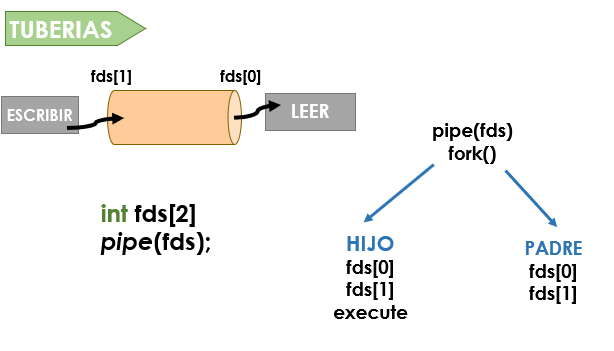
\includegraphics[width=0.9\textwidth]{Practica6/Images/General/Tuberias.PNG}
          \end{figure}
          Permite enviar la salida de uno comando a otro. Una \textsf{tuberia}, como suele decirse, puede redirigir la salida estándar, la entrada o el error de un proceso a otro para su posterior procesamiento.

          La sintaxis para el omando es con el caracter $|$ entre dos comandos:

          \begin{figure}[h!]
                \centering
               
\includegraphics[width=0.9\textwidth]{Practica6/Images/General/Comandos.PNG}
          \end{figure}

          No se puede acceder a la tubería a través de otra sesión, se crea temporalmenta para acomodar la ejecución del \textbf{Comando 1} y redirigir la salida estándar. Se elimina después de la ejecución exitosa.

          Una tubería con nombre puede durar hasta que el sistema esté en funcionamiento o hasta que se elimine. Es un archivo especial que sigue el mecanismo \textbf{FIFO} $($ Primero en entrar, primero en salir$)$. Se puede utilizar como un archivo normal, es decir, puede escribir, leer, abrir o cerrar. Para crear una tubería con nombre se usa el comando:

          \begin{figure}[h!]
                \centering
               
\includegraphics[width=0.9\textwidth]{Practica6/Images/General/mkfifo.PNG}
          \end{figure}

        \item[\Checkmark] \textbf{shmget()}
        \item[\Checkmark] \textbf{shmat()}
      \end{itemize}
      
      % /////////////////////////////////////////////////////////////////////
      %                              SECCION DE WINDOWS
      % /////////////////////////////////////////////////////////////////////
          
      \subsubsection{Sección Windows:}

      		         
    % //////////////////////////////////////////////////////////////////////////////////
    % 		      				CODIGOS FUENTE DE LOS PROGRAMAS DESARROLLADOS
    % /////////////////////////////////////////////////////////////////////////////////

    \subsection{Códigos fuente de los programas desarrollados}
  	
      % /////////////////////////////////////////////////////////////////////
      %                              SECCION DE LINUX
      % /////////////////////////////////////////////////////////////////////

    	\subsubsection{Sección Linux}

      % /////////////////////////////////////////////////////////////////////
      %                              SECCION DE WINDOWS
      % /////////////////////////////////////////////////////////////////////
    
    	\subsubsection{Sección Windows}
      	
\newpage

    % ////////////////////////////////////////////////////////////////////////////////////////////////////
    %                      PANTALLAS DE EJECUCIÓN DE LOS PROGRAMAS DESARROLLADOS
    % ////////////////////////////////////////////////////////////////////////////////////////////////////      

    \subsection{Pantallas de ejecución de los programas desarrollados}
      		
      % /////////////////////////////////////////////////////////////////////
      %                              SECCION DE LINUX
      % /////////////////////////////////////////////////////////////////////
        
  		\subsubsection{Sección Linux:}
            			 
      % /////////////////////////////////////////////////////////////////////
      %                              SECCION DE WINDOWS
      % /////////////////////////////////////////////////////////////////////
        
	    \subsubsection{Sección Windows:}


  % /////////////////////////////////////////////////////////////////////////////////////////////////////
  %                                             OBSERVACIONES
  % ////////////////////////////////////////////////////////////////////////////////////////////////////
  
  \section{Observaciones}


  % ////////////////////////////////////////////////////////////////////////////////////////////////////
  %                                          ANALISIS CRITICO
  % ////////////////////////////////////////////////////////////////////////////////////////////////////
	
	\section{Análisis Crítico}

  % ///////////////////////////////////////////////////////////////////////////////////////////////////
  %                                            CONCLUSIONES
  % ///////////////////////////////////////////////////////////////////////////////////////////////////
	
	\section{Conclusiones}


\end{document}